% Single-step SDE PPO: bandit reduction, exact credit assignment, and a
% per-sample implementation design for Flow-Factory.
% Compile: pdflatex single_step_sde_ppo.tex (run twice for refs / toc / hyperref).
% Requires: tikz, algorithm, algpseudocode, booktabs, amsmath, amsthm, hyperref.
\documentclass[11pt]{article}

\usepackage[utf8]{inputenc}
\usepackage[T1]{fontenc}
\usepackage{lmodern}
\usepackage[a4paper,margin=1in]{geometry}
\usepackage{amsmath,amssymb,amsthm,bm}
\usepackage{booktabs}
\usepackage{array}
\usepackage{enumitem}
\usepackage{caption}
\usepackage{xcolor}
\usepackage{algorithm}
\usepackage{algpseudocode}
\usepackage{tikz}
\usetikzlibrary{arrows.meta,positioning,shapes.geometric,calc,fit,backgrounds}
\usepackage[colorlinks=true,linkcolor=blue,citecolor=blue,urlcolor=teal]{hyperref}

% Let TeX absorb long \texttt tokens / inline paths at line ends without overfull boxes.
\emergencystretch=3em

\theoremstyle{plain}
\newtheorem{proposition}{Proposition}
\theoremstyle{remark}
\newtheorem{remark}{Remark}

\tikzset{
  st/.style={draw, circle, minimum size=0.95cm, fill=gray!8, font=\small},
  stsde/.style={draw, circle, minimum size=0.95cm, fill=orange!18, font=\small},
  box/.style={draw, rounded corners, align=center, minimum height=0.9cm,
              text width=3.0cm, fill=blue!5, font=\small},
  flow/.style={-{Stealth[length=2.3mm]}, thick},
  odeflow/.style={-{Stealth[length=2.3mm]}, thick, gray},
  sdeflow/.style={-{Stealth[length=2.6mm]}, very thick, orange!75!black},
}

\newcommand{\zt}{\bm{z}}
\newcommand{\E}{\mathbb{E}}
\newcommand{\R}{\mathbb{R}}
\newcommand{\Var}{\mathrm{Var}}
\newcommand{\Vphi}{V_\phi}
\newcommand{\eps}{\bm{\epsilon}}

\title{\textbf{Single-Step SDE PPO for Flow-Matching Models}\\[2pt]
\large Bandit Reduction, Exact Credit Assignment, and a Per-Sample Design (Flow-Factory)}
\author{Flow-Factory}
\date{\today}

\begin{document}
\maketitle

\begin{abstract}
Flow-Factory's critic-based PPO currently rolls out a \emph{full} SDE trajectory:
every denoising step injects noise, and Generalized Advantage Estimation (GAE)
distributes the terminal reward over all steps. This note develops an alternative
regime in which \emph{exactly one} denoising step $k$ is stochastic (SDE) and all
other steps are deterministic (ODE). We show this reduces the denoising MDP to a
\emph{contextual bandit} at step $k$: the state is the deterministic ODE-mapped latent
$\zt_k$, the action is the single SDE transition $\zt_{k+1}\sim\pi_\theta(\cdot\mid
\zt_k)$, and the reward is a \emph{deterministic} function of that action. The
deterministic tail makes the action-value exact, $Q(\zt_k,\zt_{k+1})=R$, so the
advantage $A=R-\Vphi(\zt_k)$ is \emph{exact} (no bootstrap/GAE bias) and the policy
gradient is a single clean term $\nabla\!\log\pi_\theta(\zt_{k+1}\mid\zt_k)\,(R-\Vphi)$.
A variance decomposition shows that, conditioned on $\zt_k$, all of $R$'s randomness is
due to the step-$k$ noise, so the credit is unconfounded---the precise sense in which
this scheme ``assigns credit correctly.'' We give the corrected advantage / value /
critic-fitting logic, show it is the $S{=}1$ special case of the existing
\texttt{compute\_gae}, and present a concrete \emph{per-sample} implementation design
(scheduler per-sample SDE mask, single-transition storage, collapsed optimize loop) so
that one rollout batch covers all timesteps. Implementation is deferred; this document
is the theory + design reference. Companion: \texttt{docs/ppo/ppo\_analysis} (the
current full-SDE trainer) and \texttt{docs/ppo/ppo\_papers\_comparison}.
\end{abstract}

\tableofcontents

\section{Motivation}
\label{sec:motivation}

In the current trainer (\texttt{docs/ppo/ppo\_analysis}) the denoising rollout is a
finite-horizon MDP over the SDE steps; \emph{every} step is stochastic, and GAE spreads
the single terminal reward $R$ across all $S$ steps. This is flexible but has two
costs for \emph{credit assignment}:

\begin{enumerate}[leftmargin=1.5em]
  \item \textbf{Confounded per-step credit.} The per-step advantage $A_s=R-\Vphi(\zt_s)$
  (the $\gamma{=}\lambda{=}1$ case) treats one Monte-Carlo $R$ as the return from
  $\zt_s$, but $R$'s value depends on the noise of \emph{all} downstream steps
  $s,\dots,S-1$. The signal attributable to the specific action at step $s$ is buried in
  the variance contributed by the other steps. With $\lambda<1$ the bootstrap
  $\Vphi(\zt_{s+1})$ removes some variance at the price of bias.
  \item \textbf{Every step trained every rollout.} The optimize loop iterates all $S$
  SDE steps (\texttt{trainers/ppo/trainer.py}), so compute scales with $S$.
\end{enumerate}

\textbf{Idea.} Make exactly one step $k$ stochastic and run the rest as ODE. Then the
final reward's randomness comes \emph{only} from step $k$, so the reward is causally and
statistically attributable to that one action---exact credit assignment---and we train
only that step (Flow-GRPO-style step reduction). Rotating $k$ across samples/iterations
trains the whole velocity field.

\paragraph{This is realizable today at the sampler level.} Flow-Factory's scheduler
already turns a step with \texttt{noise\_level}${=}0$ into an exact ODE step: for
Flow-SDE the transition mean collapses to $\zt_{i+1}=\zt_i+\bm v_\theta\,\mathrm dt$ and
no noise is injected (\texttt{scheduler/flow\_match\_euler\_discrete.py}). Selecting a
single SDE step per rollout (\texttt{num\_sde\_steps}${=}1$) therefore already produces
the single-SDE trajectory, and---as \S\ref{sec:fitting} shows---\texttt{compute\_gae}
already collapses to the exact single-step advantage. What is missing is (i) the theory
that justifies and characterizes this regime, and (ii) a \emph{per-sample} $k$ so a
single batch covers all timesteps (today the SDE step is one global choice per epoch).

\section{Setup: the Denoising Chain with SDE and ODE Steps}
\label{sec:setup}

A rollout produces latents $\zt_0\to\zt_1\to\cdots\to\zt_T$, with $\zt_0\sim\mathcal
N(0,\bm I)$ the initial noise and $\zt_T$ decoded to the sample $\bm x=\mathrm{dec}(\zt_T)$
scored by the (terminal) reward $R=\sum_m w_m r_m(\bm x)$. Step $i$ uses the network's
velocity prediction $\bm v_\theta(\zt_i,t_i)$. Two transition types:

\begin{align}
\text{ODE (deterministic):}\quad
  &\zt_{i+1}=\zt_i+\bm v_\theta(\zt_i,t_i)\,\mathrm dt_i, \label{eq:ode}\\
\text{SDE (stochastic):}\quad
  &\zt_{i+1}=\bm\mu_\theta(\zt_i,t_i)+\sigma_i\,\eps_i,\quad \eps_i\sim\mathcal N(0,\bm I),
  \label{eq:sde}
\end{align}
where $\bm\mu_\theta$ is the Flow-SDE mean and $\sigma_i=\texttt{std\_dev\_t}\cdot
\sqrt{-\mathrm dt_i}$. Crucially, the scheduler's Flow-SDE mean satisfies
$\bm\mu_\theta\to \zt_i+\bm v_\theta\,\mathrm dt_i$ and $\sigma_i\to0$ as
$\texttt{noise\_level}\to0$, so \eqref{eq:sde} \emph{reduces exactly} to \eqref{eq:ode}
when noise is switched off. The per-step Gaussian density of \eqref{eq:sde},
\begin{equation}
\label{eq:logprob}
\log\pi_\theta(\zt_{i+1}\mid\zt_i,t_i)
  = -\frac{\lVert \zt_{i+1}-\bm\mu_\theta(\zt_i,t_i)\rVert^2}{2\sigma_i^2}
    -\log\sigma_i - \tfrac12\log 2\pi
\quad(\text{per-dimension mean}),
\end{equation}
is what the rollout stores and what the policy ratio recomputes; it is well-defined only
when $\sigma_i>0$ (an SDE step).

\paragraph{Single-step SDE.} Fix one index $k\in\{0,\dots,T-1\}$. Use \eqref{eq:sde} at
$i=k$ and \eqref{eq:ode} for all $i\neq k$. Write the deterministic ODE solution
operators
\begin{equation}
\Phi_{0\to k}:\ \zt_0\mapsto\zt_k,
\qquad
\Phi_{k+1\to T}:\ \zt_{k+1}\mapsto\zt_T,
\end{equation}
both deterministic functions of $\theta$. Figure~\ref{fig:traj} contrasts the full-SDE
and single-SDE trajectories.

\begin{figure}[h]
\centering
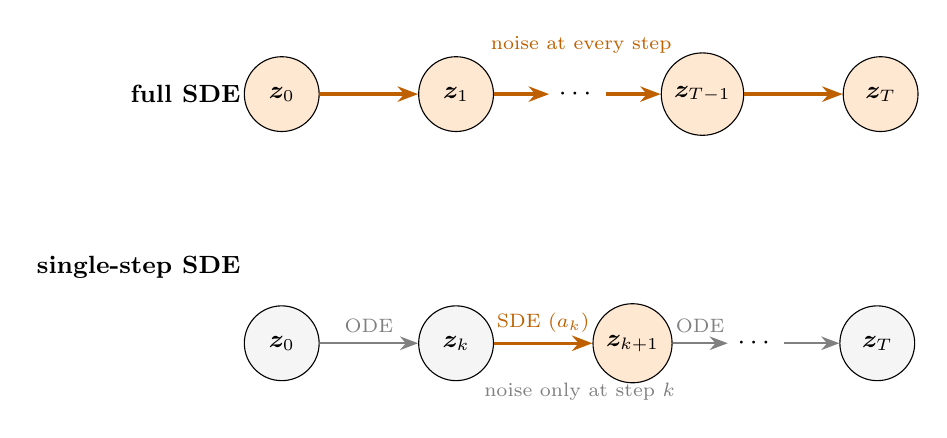
\begin{tikzpicture}[node distance=1.25cm]
  % Full SDE row
  \node[font=\small\bfseries, anchor=east] at (-0.4,0) (lblA) {full SDE};
  \node[stsde] (a0) {$\zt_0$};
  \node[stsde, right=of a0] (a1) {$\zt_1$};
  \node[right=0.7cm of a1] (ad) {$\cdots$};
  \node[stsde, right=0.7cm of ad] (aS1) {$\zt_{T-1}$};
  \node[stsde, right=of aS1] (aS) {$\zt_T$};
  \draw[sdeflow] (a0)--(a1); \draw[sdeflow] (a1)--(ad);
  \draw[sdeflow] (ad)--(aS1); \draw[sdeflow] (aS1)--(aS);
  % Single SDE row
  \node[font=\small\bfseries, anchor=east] at (-0.4,-2.2) (lblB) {single-step SDE};
  \node[st, below=2.2cm of a0] (b0) {$\zt_0$};
  \node[st, right=of b0] (bk) {$\zt_k$};
  \node[stsde, right=of bk] (bk1) {$\zt_{k+1}$};
  \node[right=0.7cm of bk1] (bd) {$\cdots$};
  \node[st, right=0.7cm of bd] (bS) {$\zt_T$};
  \draw[odeflow] (b0)-- node[above,font=\scriptsize,gray]{ODE} (bk);
  \draw[sdeflow] (bk)-- node[above,font=\scriptsize]{SDE ($a_k$)} (bk1);
  \draw[odeflow] (bk1)-- node[above,font=\scriptsize,gray]{ODE} (bd);
  \draw[odeflow] (bd)-- (bS);
  \node[font=\scriptsize, orange!75!black] at ($(a0)!0.5!(aS)+(0,0.62)$) {noise at every step};
  \node[font=\scriptsize, gray] at ($(b0)!0.5!(bS)+(0,-0.62)$) {noise only at step $k$};
\end{tikzpicture}
\caption{Top: the current full-SDE rollout (every transition stochastic). Bottom: the
single-step SDE rollout---deterministic ODE except at step $k$, the sole source of
randomness downstream of $\zt_0$.}
\label{fig:traj}
\end{figure}

\section{Single-Step SDE Reduces Denoising to a Contextual Bandit}
\label{sec:bandit}

With noise only at $k$, the trajectory has a single stochastic decision. Define the
\emph{contextual bandit}:
\begin{center}
\begin{tabular}{ll}
\toprule
context (state) & $s=\zt_k=\Phi_{0\to k}(\zt_0)$ \quad(deterministic in $\zt_0$)\\
action & $a=\zt_{k+1}\sim\pi_\theta(\cdot\mid \zt_k,t_k)=\mathcal N(\bm\mu_\theta,\sigma_k^2\bm I)$\\
reward & $R=\rho(\zt_{k+1}):=r\big(\mathrm{dec}(\Phi_{k+1\to T}(\zt_{k+1}))\big)$ \quad(deterministic in $a$)\\
\bottomrule
\end{tabular}
\end{center}
The horizon-$T$ MDP collapses to one decision: observe $\zt_k$, draw the action
$\zt_{k+1}$, receive the deterministic reward $\rho(\zt_{k+1})$. The initial noise
$\zt_0$ only enters through the context $\zt_k$. Figure~\ref{fig:bandit} summarizes.

\begin{figure}[h]
\centering
\resizebox{\textwidth}{!}{%
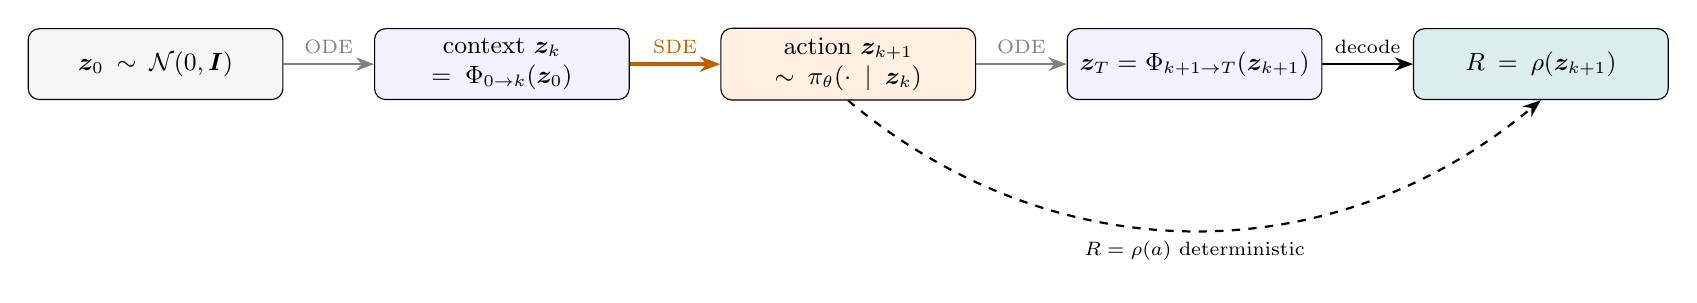
\begin{tikzpicture}[node distance=0.7cm and 1.15cm]
  \node[box, fill=gray!8] (z0) {$\zt_0\sim\mathcal N(0,\bm I)$};
  \node[box, right=of z0] (zk) {context $\zt_k$\\ $=\Phi_{0\to k}(\zt_0)$};
  \node[box, right=of zk, fill=orange!12] (act) {action $\zt_{k+1}$\\ $\sim\pi_\theta(\cdot\mid\zt_k)$};
  \node[box, right=of act] (tail) {$\zt_T=\Phi_{k+1\to T}(\zt_{k+1})$};
  \node[box, right=of tail, fill=teal!14] (rew) {$R=\rho(\zt_{k+1})$};
  \draw[odeflow] (z0)-- node[above,font=\scriptsize,gray]{ODE} (zk);
  \draw[sdeflow] (zk)-- node[above,font=\scriptsize]{SDE} (act);
  \draw[odeflow] (act)-- node[above,font=\scriptsize,gray]{ODE} (tail);
  \draw[flow] (tail)-- node[above,font=\scriptsize]{decode} (rew);
  \draw[flow, dashed] (act.south) to[out=-40,in=-140] node[below,font=\scriptsize]{$R=\rho(a)$ deterministic} (rew.south);
\end{tikzpicture}%
}
\caption{The single-step SDE process as a contextual bandit. Everything except the
step-$k$ transition is deterministic, so $R$ is a deterministic function $\rho$ of the
action $\zt_{k+1}$.}
\label{fig:bandit}
\end{figure}

\section{Exact Value and Advantage (Deterministic-Tail Identity)}
\label{sec:exact}

Define the state and action values for this bandit:
\begin{equation}
Q^\pi(\zt_k,a)=\E[R\mid \zt_k, \zt_{k+1}=a],
\qquad
\Vphi(\zt_k,t_k)\approx V^\pi(\zt_k)=\E_{a\sim\pi_\theta(\cdot\mid\zt_k)}[R].
\end{equation}

\begin{proposition}[Deterministic tail $\Rightarrow$ exact advantage]
\label{prop:exact}
If steps $k{+}1,\dots,T{-}1$ are deterministic (ODE), then for the realized action
$a=\zt_{k+1}$,
\[
Q^\pi(\zt_k,a)=R,\qquad V^\pi(\zt_{k+1},t_{k+1})=R,
\]
and the action advantage is \emph{exact},
\[
A(\zt_k,a)=Q^\pi(\zt_k,a)-V^\pi(\zt_k)=R-V^\pi(\zt_k,t_k),
\]
with no bootstrap or GAE truncation error. Moreover $\E_{a\sim\pi_\theta(\cdot\mid\zt_k)}
[A(\zt_k,a)\mid\zt_k]=0$.
\end{proposition}

\begin{proof}
Given $\zt_{k+1}$, the tail $\zt_T=\Phi_{k+1\to T}(\zt_{k+1})$ and $R=\rho(\zt_{k+1})$
are deterministic, so $Q^\pi(\zt_k,a)=\E[R\mid \zt_{k+1}=a]=\rho(a)=R$. The post-action
state $\zt_{k+1}$ is terminal-equivalent: its value
$V^\pi(\zt_{k+1})=\E[R\mid\zt_{k+1}]=\rho(\zt_{k+1})=R$. The advantage is
$Q-V=R-V^\pi(\zt_k)$. Finally $\E_a[Q^\pi(\zt_k,a)]=\E_a[R]=V^\pi(\zt_k)$, so the
advantage is mean-zero under the policy.
\end{proof}

Contrast with full SDE, where $Q^\pi(\zt_s,a_s)=\E[R\mid\zt_s,a_s]$ still averages over
the downstream noise $\eps_{s+1},\dots,\eps_{S-1}$; using a single $R$ as the return is a
\emph{high-variance} estimate of $Q$, and bootstrapping ($\lambda<1$) trades that
variance for bias. The deterministic tail removes both: $R$ \emph{is} $Q$.

\section{Single-Step Policy Gradient and PPO Objective}
\label{sec:pg}

Conditioned on $\zt_0$, only the step-$k$ transition carries a probability density; the
ODE steps are deterministic (Dirac) and contribute no score term. Following the standard
diffusion-policy-gradient construction (DDPO / Flow-GRPO), where the action is the next
latent and the dynamics ``$s_{i+1}=a_i$'' are parameter-free, the gradient is the single
term
\begin{equation}
\label{eq:pg}
\nabla_\theta J_k(\theta)
= \E_{\zt_0,\,\eps_k}\!\Big[\nabla_\theta\log\pi_\theta(\zt_{k+1}\mid\zt_k,t_k)\,
   \big(R-\Vphi(\zt_k,t_k)\big)\Big].
\end{equation}
The clipped PPO surrogate, with ratio $\rho_k=\exp\!\big(\log\pi_\theta(\zt_{k+1}\mid
\zt_k)-\log\pi_{\mathrm{old}}(\zt_{k+1}\mid\zt_k)\big)$ and $\hat A=R-\Vphi$ (clamped /
whitened), is
\begin{equation}
\label{eq:ppo}
\mathcal L^{\text{pol}}_k=-\,\E\big[\min(\rho_k\hat A,\ \mathrm{clip}(\rho_k,1{+}c_-,1{+}c_+)\,\hat A)\big].
\end{equation}

\begin{remark}[What this gradient does and does not capture]
Like DDPO/Flow-GRPO, \eqref{eq:pg} treats the rollout latents as \emph{given states} and
differentiates only through the (single) stochastic transition; the cross-step pathwise
dependence of the deterministic ODE steps on $\theta$ is intentionally not
differentiated. Because $\bm v_\theta$ is shared across all noise levels, applying
\eqref{eq:pg} at step $k$ improves the policy slice $\bm v_\theta(\cdot,t_k)$; rotating
$k$ over training (\S\ref{sec:coverage}) trains the whole field. The improvement over
full-SDE is not the estimator family (still score-function with a baseline) but that the
\emph{within-step credit is exact} (Prop.~\ref{prop:exact}).
\end{remark}

\section{Why the Credit Assignment Is Correct (Variance Decomposition)}
\label{sec:credit}

Take the law of total variance for the single-SDE process, conditioning on the context
$\zt_k$:
\begin{equation}
\Var(R)=\underbrace{\E_{\zt_k}\!\big[\Var(R\mid\zt_k)\big]}_{\text{within-action (step $k$)}}
       +\underbrace{\Var_{\zt_k}\!\big(\E[R\mid\zt_k]\big)}_{\text{across contexts ($\zt_0$)}}.
\end{equation}
Conditioned on $\zt_k$, $R=\rho(\bm\mu_\theta(\zt_k)+\sigma_k\eps_k)$ depends on a single
random variable $\eps_k$, so $\Var(R\mid\zt_k)$ is \emph{entirely} the effect of the
step-$k$ action. The baseline $\Vphi(\zt_k)=\E[R\mid\zt_k]$ removes the second
(across-context) term, leaving the advantage
\begin{equation}
\hat A=R-\Vphi(\zt_k),\qquad \E[\hat A\mid\zt_k]=0,\qquad \Var(\hat A\mid\zt_k)=\Var(R\mid\zt_k),
\end{equation}
which is a zero-mean, variance-minimal (baseline = conditional mean) and---critically---
\emph{unconfounded} estimate of how much this action beat the average at step $k$.

For full SDE, the analogous per-step quantity $R-\Vphi(\zt_s)$ has
$\Var(R\mid\zt_s)=\sum_{j\ge s}(\text{contribution of }\eps_j)$: the credit for step $s$
is mixed with the noise of all later steps. Single-step SDE collapses that sum to the one
term that belongs to step $k$. This is the precise sense of ``the reward's return must
come from this one SDE step.''

\section{Corrected Advantage / Value / Critic-Fitting Logic}
\label{sec:fitting}

The single-SDE regime replaces the multi-step GAE machinery with a one-step bandit
target. Concretely, per rollout sample $i$ with SDE step $k_i$:

\begin{itemize}[leftmargin=1.5em]
  \item \textbf{Advantage:} $\hat A_i = R_i - \Vphi(\zt_{k_i},t_{k_i})$, then (optionally)
  globally whitened across the batch, exactly as today
  (\texttt{normalize\_advantage} $\to$ \texttt{whiten}). \emph{No GAE recursion}; no
  $\gamma,\lambda$.
  \item \textbf{Value target (return):} $G_i = R_i$ (Monte-Carlo, and by
  Prop.~\ref{prop:exact} \emph{exact}, not an approximation). Critic loss
  $\mathcal L^{\text{val}}_i=\tfrac12(\Vphi(\zt_{k_i},t_{k_i})-R_i)^2$, with the existing
  optional PPO value-clip around the old value (\texttt{value\_clip\_range}).
  \item \textbf{Critic semantics change.} The critic now learns the expected reward of a
  \emph{single} exploratory step from $(\zt,t)$ followed by deterministic integration
  (i.e.\ $\Vphi(\zt,t)=\E[R\mid\zt,t]$ under the single-SDE law). This differs from the
  full-SDE critic, which marginalizes over \emph{all} downstream SDE noise; the
  single-SDE target has strictly lower variance.
\end{itemize}

\paragraph{It is the $S{=}1$ collapse of \texttt{compute\_gae}.} The existing
\texttt{trainers/ppo/gae.py} already yields exactly this when there is one trained step.
With values $V\in\R^{B\times1}$ and terminal reward $R$, the backward recursion runs once
at $s=0=S-1$: $r=R$, $V_{\text{next}}=0$, $\delta=R-V[:,0]$, $A[:,0]=\delta=R-V$, and
$G=A+V=R$. So the corrected logic is not a new estimator but a \emph{first-class}
treatment of the single-step case (with per-sample $k$ and a collapsed loop), which also
removes the $\gamma{=}\lambda{=}1$ / contiguous-trajectory caveats that the full-SDE GAE
documents.

\section{Coverage: Per-Sample $k$ as Randomized-Coordinate Policy Gradient}
\label{sec:coverage}

A fixed $k$ trains only the slice $\bm v_\theta(\cdot,t_k)$. Sampling $k$ (per sample, or
per prompt-group) from a distribution $q$ over steps and optimizing the mixture
\begin{equation}
\max_\theta\ \E_{k\sim q}\big[J_k(\theta)\big]
\end{equation}
covers all timesteps. Because each rollout's gradient \eqref{eq:pg} updates the step it
sampled, this is a \emph{randomized-coordinate} policy gradient over denoising steps: one
batch with per-sample $k_i$ touches every coordinate, keeping both the policy and the
critic (\S\ref{sec:fitting}) fresh across all noise levels. We recommend $q=\mathrm{Unif}
\{0,\dots,T-2\}$ (exclude the final step, which the scheduler already treats as the
deterministic readout) unless reward sensitivity is known to concentrate at particular
noise levels, in which case $q$ can be tilted.

\begin{remark}[Why per-sample, not per-epoch]
Today \texttt{current\_sde\_steps}/\texttt{train\_timesteps} is one global choice per
epoch (seeded by \texttt{epoch+seed}), so a single-SDE epoch would train one timestep and
the critic would see one $t$ per epoch. Per-sample $k_i$ restores full timestep coverage
each batch, which is both statistically (lower-variance field estimate) and practically
(fresh critic baseline) preferable.
\end{remark}

\section{Train/Deploy Sampler Mismatch}
\label{sec:traindeploy}

Single-step SDE is an \emph{exploration} distribution: it perturbs the ODE trajectory at
one point to obtain a gradient, but deployment typically uses pure ODE (or a chosen SDE
schedule). The marginal law of $\zt_T$ under ``SDE-at-$k$'' differs from full-ODE and
full-SDE sampling. This is benign for fine-tuning the shared field $\bm v_\theta$---the
perturbation is local and, as the noise level $\to0$, vanishes---but two points deserve
care: (i) the exploration scale $\sigma_k$ (\texttt{noise\_level}) controls a
bias--variance trade-off (too small $\Rightarrow$ weak signal; too large $\Rightarrow$
states far from the deployment manifold); (ii) as the policy drifts, the single-step
perturbation should remain ``consistent'' with the ODE flow it perturbs---the same
consistency concern formalized by DiffAC~\cite{zhou2024diffac}. In practice, choosing $k$
uniformly and a moderate \texttt{noise\_level} keeps the exploration close to the
deployment trajectory.

\section{Relation to Existing Methods}
\label{sec:relations}

\begin{itemize}[leftmargin=1.5em]
  \item \textbf{Flow-GRPO}~\cite{flowgrpo}: also reduces trained steps by subsampling SDE
  steps, but uses a \emph{group-relative} (critic-free) advantage broadcast to those
  steps. Single-step SDE PPO uses a \emph{learned per-state} baseline $\Vphi(\zt_k)$ and an
  \emph{exact single-action} advantage; with one SDE step the ``which steps to train''
  question becomes ``which one step,'' answered per sample.
  \item \textbf{Current full-SDE PPO} (\texttt{docs/ppo/ppo\_analysis}): GAE over all
  steps; value marginalizes all downstream noise; per-step credit via bootstrap. Single
  step makes $A=R-\Vphi$ exact and drops the multi-step loop.
  \item \textbf{Perturbed-state critic follow-up} (\texttt{docs/ppo/ppo\_analysis},
  \S``DiffAC-style perturbed-state critic''): complementary---it widens \emph{critic}
  coverage by re-noising clean samples, and can be combined here to keep $\Vphi$ accurate
  across all $t$ even when the \emph{policy} trains a single step.
\end{itemize}

\section{Implementation Design (Per-Sample SDE Step)}
\label{sec:impl}

This section specifies the code changes; \textbf{they are deferred} (to be implemented
after this theory is reviewed). The design keeps the existing rollout/storage where
possible and adds a per-sample SDE step plus a collapsed (bandit) optimize path.

\subsection{Scheduler: per-sample SDE mask + safe log-prob}
Files under \texttt{scheduler/}: \texttt{flow\_match\_euler\_discrete.py}, the mirror
\texttt{unipc\_multistep.py}, and the contract \texttt{abc.py}.
\begin{itemize}[leftmargin=1.5em]
  \item Hold a per-sample step assignment $\bm k\in\{0,\dots,T-1\}^{B}$ (a buffer set per
  rollout). Add a setter, e.g. \texttt{set\_per\_sample\_sde\_steps(k)}.
  \item Make \texttt{get\_noise\_level\_for\_timestep(t)} return a \emph{$(B,)$ tensor}:
  \texttt{noise\_level} where $t=t_{k_i}$ else $0$. The Flow-SDE \texttt{step()} already
  broadcasts a per-sample \texttt{noise\_level} via \texttt{to\_broadcast\_tensor}, so the
  mean/noise math in \eqref{eq:sde} is unchanged (samples with $0$ collapse to ODE).
  \item \textbf{Safe log-prob.} \eqref{eq:logprob} divides by $\sigma_i$; for non-SDE
  samples $\sigma_i{=}0$. Guard the division (e.g. compute on a safe denominator and mask
  the non-SDE rows to $0$/NaN-free) so a batched step with mixed SDE/ODE rows does not
  divide by zero.
\end{itemize}

\subsection{Rollout: per-sample gate}
Files: the shared inference path and per-adapter loops (e.g.
\texttt{models/stable\_diffusion/sd3\_5.py}). Today the loop computes a scalar
\texttt{current\_noise\_level = get\_noise\_level\_for\_timestep(t)} and gates
\texttt{current\_compute\_log\_prob = compute\_log\_prob and current\_noise\_level > 0}.
With per-sample $k$, every step has \emph{some} SDE rows, so:
\begin{itemize}[leftmargin=1.5em]
  \item Replace the scalar gate by a per-sample-aware one (compute log-prob whenever
  \emph{any} row is SDE at this step), ideally via a small scheduler helper
  (\texttt{should\_compute\_log\_prob(t)}) to minimize per-adapter churn (constraint:
  changes to shared infra affect all adapters).
  \item Continue storing the full \texttt{all\_latents}; store per-step
  \texttt{log\_probs} with the non-SDE rows masked. Each sample contributes exactly one
  real log-prob (at its $k_i$).
\end{itemize}

\subsection{Sample storage: a single transition per sample}
Rather than rely on the shared \texttt{latent\_index\_map} (which assumes a common set of
trajectory positions across the batch), gather \emph{per sample} the one transition it
trains on: $(\zt_{k_i},\,t_{k_i},\,\zt_{k_i+1},\,\log\pi_{\mathrm{old}}(\zt_{k_i+1}\mid
\zt_{k_i}))$ plus the scalar $R_i$. This is a fixed-size per-sample record (independent
of $k_i$), simplifying the feedback/optimize code.

\subsection{Feedback and optimize: collapse to the bandit update}
Files: \texttt{trainers/ppo/trainer.py}, \texttt{trainers/ppo/gae.py}.
\begin{itemize}[leftmargin=1.5em]
  \item \texttt{prepare\_feedback}: compute $R_i$ (reuse
  \texttt{\_compute\_terminal\_rewards}); $V^{\text{old}}_i=\Vphi(\zt_{k_i},t_{k_i})$
  (one query per sample, replacing the per-step \texttt{\_compute\_old\_values} loop);
  $\hat A_i=R_i-V^{\text{old}}_i$ then \texttt{whiten}; store $\hat A_i$, $G_i=R_i$,
  $V^{\text{old}}_i$ as \emph{per-sample scalars} (replacing the $(B,S)$ tensors and the
  \texttt{compute\_gae} call).
  \item \texttt{optimize}: drop the \texttt{for timestep\_index in sorted\_ts} loop. Per
  micro-batch, one PPO-clip update \eqref{eq:ppo} at each sample's $(\zt_{k_i},t_{k_i})$
  using its stored $\zt_{k_i+1}$, and one critic step
  $\Vphi(\zt_{k_i},t_{k_i})\to R_i$. The critic warmup / re-warmup paths
  (\texttt{\_fit\_critic\_only}) collapse identically (one value query per sample).
  \item GAS bookkeeping: \texttt{get\_num\_train\_timesteps} returns $1$ trained step per
  sample (instead of \texttt{num\_sde\_steps}); update the auto-GAS multiplier accordingly.
\end{itemize}

\subsection{Hparams and config}
Files: \texttt{hparams/scheduler\_args.py} and \texttt{hparams/training\_args/ppo.py};
example under \texttt{examples/ppo/lora/sd3\_5/}.
\begin{itemize}[leftmargin=1.5em]
  \item Add \texttt{sde\_step\_selection: \{global, per\_sample\}} (default \texttt{global}
  preserves current behavior) and the per-sample $k$ distribution $q$ (e.g.
  \texttt{uniform}); fail-fast validation: per-sample mode requires
  \texttt{dynamics\_type=Flow-SDE} and a single SDE step per sample.
  \item Add an example \texttt{examples/ppo/lora/sd3\_5/single\_sde.yaml}
  (\texttt{num\_inference\_steps} unchanged; one SDE step per sample; advantage whitening
  on; value-clip optional).
\end{itemize}

\subsection{Pseudocode}

\begin{algorithm}[H]
\caption{Per-sample single-step SDE PPO (one optimize round)}
\label{alg:single-sde}
\begin{algorithmic}[1]
\State \textbf{Rollout:} sample $k_i\sim q$ per sample; run $T$-step generation with ODE
       everywhere except step $k_i$ for sample $i$ (per-sample \texttt{noise\_level} mask).
\State \quad store per sample: $\zt_{k_i},\,t_{k_i},\,\zt_{k_i+1},\,
       \log\pi_{\mathrm{old}}(\zt_{k_i+1}\mid\zt_{k_i})$; decode $\zt_T^{(i)}$.
\State \textbf{Reward:} $R_i\gets$ terminal weighted-sum score of $\mathrm{dec}(\zt_T^{(i)})$.
\State \textbf{Feedback (no grad):} $V^{\text{old}}_i\gets \Vphi(\zt_{k_i},t_{k_i})$;\quad
       $\hat A_i\gets R_i-V^{\text{old}}_i$;\quad $\hat A\gets\textsc{Whiten}(\hat A)$;\quad $G_i\gets R_i$.
\For{inner epoch, micro-batch}
  \State \textbf{Critic:} $V_i\gets\Vphi(\zt_{k_i},t_{k_i})$;\ \
         $\mathcal L^{\text{val}}=\tfrac12\big(V_i-G_i\big)^2$ (optional value-clip);\ backward; step critic opt.
  \State \textbf{Policy:} recompute $\log\pi_\theta(\zt_{k_i+1}\mid\zt_{k_i})$;\ \
         $\rho_i=\exp(\log\pi_\theta-\log\pi_{\mathrm{old}})$;
  \State \quad $\mathcal L^{\text{pol}}=-\min(\rho_i\hat A_i,\ \mathrm{clip}(\rho_i,1{+}c_-,1{+}c_+)\hat A_i)$;\ backward; step policy opt.
\EndFor
\end{algorithmic}
\end{algorithm}

\noindent Note the inner body has \emph{no} timestep loop---one transition per sample---
which is the compute reduction relative to the full-SDE loop over \texttt{sorted\_ts}.

\section{Summary}
\label{sec:summary}
Injecting SDE noise at a single denoising step turns diffusion RL into a contextual
bandit whose deterministic tail makes the advantage $A=R-\Vphi(\zt_k)$ \emph{exact}
(Prop.~\ref{prop:exact}) and whose reward variance, conditioned on the context, is
attributable solely to that step (\S\ref{sec:credit}). The corrected logic is the
$S{=}1$ collapse of our existing GAE, made first-class with per-sample $k$ for full
timestep coverage (\S\ref{sec:coverage}). The implementation (\S\ref{sec:impl}) is a
per-sample SDE mask in the scheduler plus a collapsed bandit optimize path, deferred to a
follow-up after this theory is reviewed.

\begin{thebibliography}{9}
\bibitem{flowgrpo}
Jie Liu et al.
\newblock Flow-GRPO: Training Flow-Matching Models via Online RL.
\newblock arXiv:2505.05470, 2025. \url{https://arxiv.org/abs/2505.05470}

\bibitem{ddpo}
Kevin Black, Michael Janner, Yilun Du, Ilya Kostrikov, Sergey Levine.
\newblock Training Diffusion Models with Reinforcement Learning (DDPO).
\newblock arXiv:2305.13301, 2023. \url{https://arxiv.org/abs/2305.13301}

\bibitem{ppo}
John Schulman, Filip Wolski, Prafulla Dhariwal, Alec Radford, Oleg Klimov.
\newblock Proximal Policy Optimization Algorithms.
\newblock arXiv:1707.06347, 2017. \url{https://arxiv.org/abs/1707.06347}

\bibitem{gae}
John Schulman, Philipp Moritz, Sergey Levine, Michael Jordan, Pieter Abbeel.
\newblock High-Dimensional Continuous Control Using Generalized Advantage Estimation.
\newblock arXiv:1506.02438, 2015. \url{https://arxiv.org/abs/1506.02438}

\bibitem{zhou2024diffac}
Xiangxin Zhou, Liang Wang, Yichi Zhou.
\newblock Stabilizing Policy Gradients for SDEs via Consistency with Perturbation Process (DiffAC).
\newblock ICML 2024; arXiv:2403.04154. \url{https://arxiv.org/abs/2403.04154}
\end{thebibliography}

\end{document}
